\lab{Algorithms}{Matrix Operations and Algorithmic Complexity}{Matrices and
Complexity}
\objective{This lesson explains basic matrix operations in Python.}

%Make a note command

Matrices form the core data structure of NumPy and SciPy.  Thus, we will explore
the ways one can manipulate matrices in Python.

Before we begin, we make a few important comments about how Python works with matrices. First of all, matrices can be represented in NumPy in two ways.  NumPy has a matrix
datatype and an array datatype.  Matrix objects are a special case of the array
object.  The main differences are that the matrix object allows for a clearer,
more matlab type syntax.  In this book, we will use arrays because most functions in python use arrays as input. We can easily convert arrays to matrices using the asmatrix()
method.  As such, all future references to matrices in the context of NumPy will
mentioned as arrays (a matrix being a 2D array).  When using arrays it is important to be sure that the dimensions are compatible.

We also note that arrays are stored row by row. This is called Row-Major. This is the opposite of MATLAB, which is Column-Major.

Finally, with all code examples in this book we assume that you have already imported the SciPy library (type \texttt{import scipy as sp} when you first open ipython).

To begin we will work with vectors. We will demonstrate a variety of methods to
create vectors. You should follow these demonstrations on your own computer and
experiment as you go.  Vectors are at least one dimensional arrays.  There are
several ways to create vectors in Python.  Try the following in IPython:

\begin{lstlisting}
: a = sp.array([1,2,3,4]); a
array([1, 2, 3, 4])
\end{lstlisting}

Notice the square brackets and the commas.  The square brackets denote a list in
Python with values separated by commas.  This is a row vector.  The \texttt{; a}
is responsible for printing the current value of \texttt{a}.  How do we make a
column vector?  We simply pass the array() method a list of lists containing a
single value each.
\begin{lstlisting}
: b = sp.array([[3],[4],[6]]); b
array([[3],
       [4],
       [6]])
\end{lstlisting}

We can also use the hstack() and vstack() methods (meaning horizontal stack and
vertical stack).
\begin{lstlisting}
: a1 = sp.hstack([5,6,7,8])
: b1 = sp.vstack([9,0,1,2])
\end{lstlisting}

We combine vectors together by placing two or more of equal dimension inside
square brackets. The technical term for this is concatenation.  Remember that
the dimensions of each array must match.  Try the following.
\begin{lstlisting}
: c = sp.concatenate(b,b1); c
\end{lstlisting}

There are several methods to automate vector creation. For example, we can build
a vector of consecutive values using the \texttt{arange()} method.

\begin{lstlisting}
: sp.arange(5)
\end{lstlisting}

Notice how the values start at zero and increment up to, but \emph{not}
including 5.  This is standard Python behaviour.  The \texttt{arange()} method
also allows us to specifiy step size
This syntax also allows us to specify step size:

\begin{lstlisting}
: sp.arange(1,3,step=0.5)
\end{lstlisting}

We can similarly use negative step sizes (note that the starting must be greater
than the endpoint).

\begin{lstlisting}
: sp.arange(3,1, step=-.5)
\end{lstlisting}

A related function is called \li{linspace()}. It allows us to specify two
endpoints and the number of equidistant values we want between the two.  Unlike
\li{arange()}, \li{linspace()} will always include both endpoints.

\begin{lstlisting}
: sp.linspace(1,2,5)
\end{lstlisting}

The \li{plot()} function uses two vectors to create a graph, the first vector
representing $x$-values and the second representing the corresponding
$y$-values.  To use \li{plot()}, we need to import the Matplotlib library.  As
an example we plot a line of slope two using the following commands (See figure
1.1):

\begin{lstlisting}
: import matplotlib.pyplot as plt
: x = sp.linspace(-2,2,20)
: plt.plot(x,2*x)
: plt.show()    
\end{lstlisting}

\begin{figure}
\begin{center}
        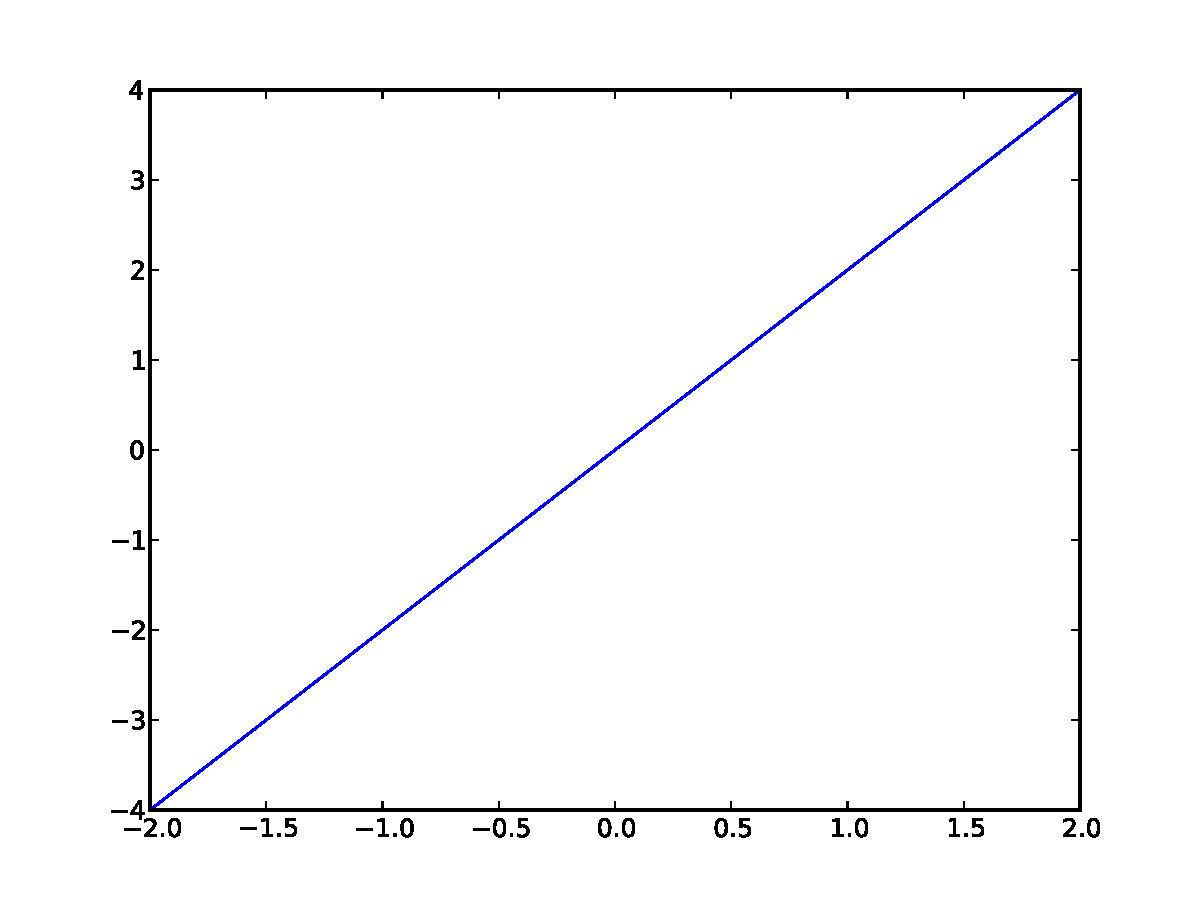
\includegraphics[scale=0.5]{./Figures/graph.pdf}
        \caption{A simple graph}
\end{center}
\end{figure}

By typing \li{plt.plot?} into the command line we can find the exact syntax and
options for the \li{plot()} function. For example we can type {\tt
plot(x,2*x,'r*')} to plot red star data points instead of a line.

\begin{problem}
Plot a line with slope three with black diamond data points. Plot for the domain
$x \in [-5,5]$. 
\end{problem}

Creating is done by concatenating vectors in the correct manner. For example:

\begin{lstlisting}
: sp.array([[1, 2, 3];[4, 5, 6];[7, 8, 9]])
\end{lstlisting}

\begin{problem}
Create a matrix showing the times table from 1 to 6. Do not enter each number
manually. Instead, create a variable \li{x = sp.arange(1,7)} and let the rows
of the matrix be multiples of $x$.
\end{problem}

Another technique for creating matrices is using outer products. An outer
product is the method of multiplying two vectors to get a matrix. For example,
if we want to make a matrix that is two repeated rows of the vector 1:5 we can
do the following:

\begin{lstlisting}
: sp.vstack([1,1])*sp.arange(1,6)
\end{lstlisting}

Here we are multiplying a $2 \times 1$ vector and a $1 \times 5$ vector, which
yields a $2 \times 5$ matrix. The two rows are identical since the entries of
the first vector are all ones.

%SciPy has an outer product function
\begin{problem}
Create the same matrix from problem 2, using outer products this time. This
implementation, although perhaps more difficult to conceptualize, makes for much
more concise code.
\end{problem}

You can also combine matrices in the same way as vectors, as long as the
dimensions match correctly, i.e. the same number of rows or the same number of
columns. Try the following:

\begin{lstlisting}
: D = sp.hstack((b, c))
: E = sp.concatenate([D.T, sp.vander(sp.arange(1,5))])
\end{lstlisting}

Here we used the \li{vander()} method, which accepts a vector of length $n$ and
creates an $n \times n$ matrix. The columns of this matrix are powers of the
input vector (evaluated point-wise). More information about the \li{vander()}
method by typing \li{sp.vander?}.

To briefly review, vectors are built using the square brackets, with semi-colons
to build columns and spaces to build rows. Matrices are built in exactly the
same way, using vectors or matrices instead of individual numbers.

Often while writing code it is necessary to know information about the
properties of an array.  The matrix properties can be accessed as follows.

\begin{lstlisting}
: E.ndim        #dimension of E
: E.nbytes      #size of E in memory (bytes)
: E.size        #total area of E (the product of the dimensions)
: E.shape       #size of E in each dimension
\end{lstlisting}

For this next problem we will need to read an array from a file.  SciPy provides
a method for loading data from text files.  We are going to load \li{bucky.csv}
as an array.
\begin{lstlisting}
: bucky = sp.loadtxt("bucky.csv", delimiter=",")
\end{lstlisting}

This array represents the connections between vertices of a truncated
isocahedron.  This soccer ball like shape is found in certain types of carbon
molecules known as fullerenes (specifically $C_{60}$, shown in shaped 
 
%---REMOVE PROBLEM?---
\begin{problem}
The bucky matrix represents the connections
between the vertices of a truncated isocahedron. This structure matches both the
structure of a standard soccer ball, and also of certain types of carbon
molecules known as fullerenes (specifically $C_{60}$, shown
in~\ref{fig:fullerene}). It is also related to the structure of the geodesic
dome. Find the size of this matrix.
\end{problem}

\begin{figure}[h!]
\begin{center}
\label{fig:fullerene}
\includegraphics[scale = .2]{./Figures/C60a.png}
\caption{The structure of the $C_{60}$ molecule.}
\end{center}
\end{figure}


To access information in an array, you put the index you wish to access inside
square brackets after the variable name. This works for both variable assignment
and retrieval.  Remember that indices start at zero in SciPy.

\begin{lstlisting}
: rand_mat = sp.random.randint(10, size=(3,5))
: rand_mat[0,0]
: rand_mat[2,2] = 37
\end{lstlisting}

The colon operator is used to retrieve an entire row or column from an array. 
For example, enter the following to get the third column of an array:

\begin{lstlisting}
: rand_mat[:,2]
\end{lstlisting}

We similarly retrieve the first row:

\begin{lstlisting}
: rand_mat[0,:]
\end{lstlisting}

Note that each retrieved row or column is returned as a single dimensional array
(meaning that row or column loses it meaning). If we want to retain the retrieved row as a column or row we can write instead \li{rand_mat[:,[2]]}.

It is also possible to retrieve multiple columns or rows at once. For example,
we retrieve the second and fourth columns of an array by entering:
\begin{lstlisting}
: rand_mat[:,[1,3]]
\end{lstlisting}

We list the entries of an array as a single dimensional array using the {\tt
flatten()} method.

\begin{lstlisting}
: rand_mat.flatten() #flattens along the rows (C like arrays)
: rand_mat. flatten('F') #flattens along the columns (Fortran like arrays)
\end{lstlisting}

The following line tells Python to retrieve the entries in the second row, from
the second column to the end:

\begin{lstlisting}
: rand_mat[1,1:]    
\end{lstlisting}

Deleting a row or column can be done by using the \li{delete()} method.  The
last argument is the axis along which to delete.  If the deletion axis is not
specified, then the array will be flattened before being returned. Here we
remove the column at index 1.
\begin{lstlisting}
: sp.delete(rand_mat, 1, 1)
\end{lstlisting}
 
\begin{problem}
Try to assign a vector of incorrect size to a piece of a matrix. What happens?
Also, try to concatenate two matrices that don't have matching dimensions. What
error message do you get? It is important to learn how to read error messages
for troubleshooting purposes.
\end{problem}

Numerical operations are by default done element-wise on arrays.  A common
mistake is to use \li{*} for matrix multiplication.  This simply multiplies
each element by a constant.  To perform matrix multiplication, SciPy provides the \li{dot()} method.  To take the transpose of an array, use the \li{.T} property.  Observe the behavior of the array operations.
\begin{lstlisting}
: b = sp.vstack([8,0,2])
: c = sp.vstack([4,2,1])
: b+c
array([[12],
       [ 2],
       [ 3]])
: b-c
array([[ 4],
       [-2],
       [ 1]])
: A = sp.array([0,4,5,4,0,2,9,4,6]).reshape((3,3))
: A*b #b is a column vector, so each row is multiplied by a constant
array([[ 0, 32, 40],
       [ 0,  0,  0],
       [18,  8, 12]])
: A*b.T #b.T is a row vector, so each column multiplied by a constant
array([[ 0,  0, 10],
       [32,  0,  4],
       [72,  0, 12]])
: sp.dot(A,b)
array([[10],
       [36],
       [84]])
: sp.power(A,2) #this is A^2
array([[ 0, 16, 25],
       [16,  0,  4],
       [81, 16, 36]])
: A/2 #notice that type is perserved.  This is integer division
array([[0, 2, 2],
       [2, 0, 1],
       [4, 2, 3]])
: A/2. #divide by a float yields an array of floats.
array([[ 0. ,  2. ,  2.5],
       [ 2. ,  0. ,  1. ],
       [ 4.5,  2. ,  3. ]])
\end{lstlisting}

The majority of elementary functions, such as \li{sin}, \li{cos}, \li{exp}, etc. act element-wise on arrays as well.  In fact, for any operation in SciPy, expect it to act element-wise unless otherwise noted.  For example:
\begin{lstlisting}
: sp.sin(sp.arange(4)*sp.pi/4)
array([ 0.        ,  0.70710678,  1.        ,  0.70710678])
\end{lstlisting}

Also, as a matter of reference, raising a value to a power is done using \li{**}. This is an convention from older programming languages that has carried over.

There are a variety of functions that let us summarize information about a given
array. For example, the \li{sum()} function returns the sum along a given axis of an array.  When an axis is not specified, all elements in the array are summed together.
\begin{lstlisting}
: B = sp.arange(9).reshape((3,3))
: sp.sum(B) #all entries are summed together
36
: sp.sum(B, axis=0) #sum each column
array([ 9, 12, 15])
: sp.sum(B, axis=1) #sum each row
array([ 3, 12, 21])     
\end{lstlisting}

Some other functions that summarize information about the entries of an array
are contained in the Table 1.1. Note that each of these functions reduces the
size of the matrix (which makes sense, since they are summarizing functions).
These functions work across columns by default, although most of them allow you
to specify an axis to work across.


\begin{table}[h!]
\begin{center}
	\begin{tabular}{|l|p{4cm}|l|}

    \hline

    Function & Description & Usage\\

    \hline

    \li{max} & Returns maximum entries & A.max(axis)\\

    \li{min} & Returns mimimum entries & A.min(axis)\\

    \li{mean} & Returns the mean & A.mean(axis)\\

    \li{scipy.median} & Returns the median & sp.median(A, axis)\\
    
    \li{std} & Returns the standard deviation & A.std(axis) \\

    \li{scipy.diff} & Returns the differences between entries & sp.diff(A, axis)\\
    
    \li{prod} & Returns the product of entries & A.prod(axis)\\
    
    \li{any} & Returns 1 if there are non-zero entries, zero otherwise & A.any(axis)\\
    
    \li{all} & Returns 1 if all entries are non-zero, zero otherwise & A.all(axis)\\

   \li{nonzero} & Returns indices of non-zero entries & A.nonzero(axis)\\

   \li{scipy.linalg.norm} & Returns the norm & norm(A, order)\\ 

    \hline

    \end{tabular}
\end{center}
\caption{Various summarizing functions}
\end{table}

These functions can be incredibly useful. For example, suppose that we want to
estimate the derivative of $sin(x^2)$. A simple approximation for a derivative
is
\[
f'(x) \approx \frac{f(x+h) - f(x)}{h}
\]

Presumably this approximation is good when $h$ is small. We use the \li{diff()}
function to perform this approximation using the following code:

\begin{lstlisting}
: h = .001
: x = sp.arange(0,sp.pi,h)
: approx = sp.diff(sin(x**2))/h
\end{lstlisting}

We have just approximated the derivative of $\sin{x^2}$ at several thousand points between $0$ and $\pi$.  The approximated derivatives are stored in the array \li{approx}.  Now let's compute the actual derivative at each point using the formula:
\[
f'(x) = 2x cos(x^2)
\]
\begin{lstlisting}
: actual = 2*sp.cos(x**2)*x;
\end{lstlisting}

Plot the approximated derivative and the actual derivative on two different
plots.  They should look almost identical.
\begin{lstlisting}
: from matplotlib import pyplot as plt
: plt.figure(1) #create an empty figure
: plt.subplot(211) #create an empty subplot in figure
: plt.plot(x, approx)
: plt.subplot(212) #create another subplot in same figure
: plt.plot(x, actual)
: plt.show()
\end{lstlisting}

\begin{problem}
Now use the \li{max()} command to find the maximum difference between the estimated derivative and the actual derivative
(the dimensions will not match exactly (why?);  fix this by removing
the last entry from one of the vectors).  Try plotting the approximation, actual deriviatives, and the error on the same graph.  What does it look like?
\end{problem}

\begin{problem}
The command \li{sp.rand()} returns an array of a specified shape with values ``randomly" selected from a uniform distribution between zero and one. Create a  vector with ten thousand entries using this command. The theoretical values for the mean($\mu$)
and standard deviation($\sigma$) of a uniformly distributed random variable
between $a$ and $b$ are
\begin{align*}
\mu &= \frac{a+b}{2} \\
\sigma &= \frac{b-a}{\sqrt{12}}
\end{align*}
These values are calculated using moment-generating functions. Use the 
\li{mean()} and \li{std()} methods on the vector you created earlier. How do these compare to the theoretical values?
\end{problem}

The canonical problem in linear algebra is solving the equation $Ax = b$ for x,
where $A$ is an $n \times n$ matrix and $b$ is a  $1 \times n$ vector.  One method for solving this equation is by calculating the matrix inverse of $A$ ($A^{-1}$) and multiplying $A^{-1}b$.  To find the inverse of an array, use the \li{linalg.inv()} method.
For example, we create a random system $Ax =b$ and solve it using the \li{inv()} method (you may check the calculations by hand):

%Excellent demonstration but needs a bit of work
\begin{lstlisting}
: A = sp.array([1,3,3,1,4,3,1,3,4]).reshape((3,3))
: b = sp.vstack([3,7,1])
: from scipy import linalg as la
: sol = sp.dot(la.inv(A),b); sol
array([[ 1.66666667],
       [ 3.33333333],
       [-2.66666667]])
\end{lstlisting}

Recall that a norm is a measurement on the size of a vector.  For example, the
Euclidean norm measures the straight line distance from the origin to the
``end'' of a vector.

\[
\norm{x} = \sqrt{x_1^2 + ... + x_n^2}
\]

If the norm of the difference of two vectors is close to zero, then they are
good approximations of each other.  The \li{linalg.norm()} function calculates the
euclidean norm of an input vector, and thus we use it to verify that our
approximation of the derivative is close to the actual derivative:
% We then verify that we have solved the system by comparing \li{A*sol} and
%\li{b} using the \li{norm} function:
\begin{lstlisting}
: la.norm(b-sp.dot(A,sol))
1.0877919644084146e-15
\end{lstlisting}

However, computing the inverse of a large matrix is difficult.  Not only that, but not all matrices have inverses.  There is a much more efficient and general way to solve $Ax=b$ in SciPy.  This method is similar to the backslash method found in MATLAB.  It is the \li{linalg.solve()} method. Compare the results obtained with the \li{linalg.solve()} method to those of the \li{linalg.inv()} method.
\begin{lstlisting}
: sol2 = la.solve(A,b); sol2
array([[ 1.66666667],
       [ 3.33333333],
       [-2.66666667]])
: la.norm(sol2-sol)
4.4408920985006262e-16
\end{lstlisting}

We mentioned that the backslash operator is more efficient than using the
function \li{inv}, meaning it returns a result faster. Create the following script to compare the efficiency of each method:

\begin{lstlisting}
import scipy as sp
from scipy import linalg as la
from timer import timer

def invMethod(A, b):
    return sp.dot(la.inv(A),b)

@tictoc(repeats=3, loops=10)
def solveMethod(A, b):
    return la.solve(A,b)
    
n = 300
A = rand(n)
b = rand(n,1)

with timer(repeats=3, loops=10) as t:
	t.time(invMethod,A,b)
	t.time(solveMethod,A,b)
	t.printTimes()
\end{lstlisting}

Now run the script. You should notice a significant difference in execution time
(you may need to scale $n$ appropriately). Are you surprised that \li{invMethod()} is significantly slower than \li{solveMethod}?  Specifically, SciPy uses the
the LU factorization and backwards substitution to solve the linear system
without any matrix inversions. %check validity

The \li{linalg.solve()} method can also be used to solve several systems at once. For example:

\begin{lstlisting}
: c = sp.rand(n, 1)
: la.solve(A, sp.c_[b,c] #sp.c_[] concatenates column vectors
\end{lstlisting}

%Explain scripts
You might now be asking why we would want to do this. We can answer this by
investigating the time it takes to solve two systems. Open a new script file and
write the following:

\begin{lstlisting}
from timer import timer
n = 3000
A = rand(n)
b = rand(n,1)
c = rand(n,1)

def multSys(A, *col_vecs):
    return la.solve(A, sp.hstack(col_vecs))
    
def singSys(A, *col_vecs):
    return [la.solve(A, x) for x in col_vecs]

with timer(repeats=3, loops=100) as t:
    t.time(multSys,A,b,c)
    t.time(singSys,A,b,c)
    t.printTimes()
\end{lstlisting}

This script creates a random $3000 \times 3000$ matrix, and two random $3000
\times 1$ vectors (you can experiment with different sizes of matrices and
vectors). It then solves the two systems of equations twice, once using two
backslash commands and the other using only one. Remember that the semi-colons
suppress the output in the script.

Now execute this script. You should notice that the first method takes about
twice as long as the second method. This is because the backslash method uses
the LU decomposition, and in the second method it only has to execute this
factorization once. This highlights the importance of understanding the
algorithms that python uses: we can solve problems much faster if we understand
what python is doing.

A number of other important operators that you will need are found in Table 1.2.
{\footnotesize
\begin{table}[h!]
\begin{center}

    \begin{tabular}{|l|p{4cm}|l|}

    \hline

    Method & Description & Usage \\

    \hline

    \li{linalg.inv()} & Matrix inverse & la.inv(A)\\

    \li{rank()} & Rank & sp.rank(A)\\

    \li{linalg.norm()} & Norm (default: 2-norm) & la.norm(A, ord)\\

    \li{linalg.expm()} & Matrix exponential & la.expm(A) \\

    \li{linalg.det()} & Determinant & la.det(A)\\

    \li{linalg.eig()} & Eigenvalue decomposition & la.eig(A)\\
    
    \li{linalg.svd()} & Singular value decomposition & la.svd(A)\\
    
    \li{linalg.lu()} & LU decomposition & la.lu(A)\\
    
    \li{linalg.qr()} & QR factorization & la.qr(A)\\
    
    \li{linalg.cholesky()} & Cholesky factorization & la.cholesky(A)\\

    \hline

    \end{tabular}
	\caption{Useful matrix operations}
\end{center} 
\end{table}}

%Explain better
\begin{problem}
The \li{linalg.solve()} method can be also used to solve overdetermined systems. This is
sometimes also known as the least squares method. The formula is $(A^TA)^{-1}A^T*b$.
Create a script to verify numerically that the \li{linalg.solve()} method and the least squares formula yield the same result. Hint: Use the \li{linalg.norm()} function to verify equality, as we did with \li{linalg.inv()} and \li{linalg.solve()}.
\end{problem}
